\newpage
\subsection{Goal}\label{subsec:goal}

The use of different representations of graphs and basic algorithms on graphs (Depth-first search and Breadth-first search).

\subsection{Formulation of the problem}\label{subsec:formulation-of-the-problem}

\paragraph{I.} Generate a random adjacency matrix for a simple undirected unweighted graph with 100 vertices and 200 edges (note that the matrix should be symmetric and contain only 0s and 1s as elements).
Transfer the matrix into an adjacency list.
Visualize the graph and print several rows of the adjacency matrix and the adjacency list.
Which purposes is each representation more convenient for?

\paragraph{II.} Use Depth-first search to find connected components of the graph and Breadth-first search to find a shortest path between two random vertices.
Analyse the results obtained.

\paragraph{III.} Describe the data structures and design techniques used within the algorithms.

\subsection{Brief theoretical part}\label{subsec:brief-theoretical-part}

A graph with no loops and no parallel edges is called a \textit{simple graph}.

\textit{Undirected graph} it is $G = (V, E)$, consisting of the set $V$ of nodes and the set $E$ of edges, which are unordered pairs of elements of $V$.

If edges in your graph have weights then your graph is said to be a \textit{weighted graph}, if the edges do not have weights, the graph is said to be \textit{unweighted}.

\textit{Adjacency matrix} is a square matrix used to represent a finite graph.
It requires $O(\lvert V \rvert^2)$ memory.

\textit{Adjacency list} is a collection of unordered lists used to represent a finite graph.
It requires $O(\lvert V \rvert + \lvert E \rvert)$ memory.

\textit{Depth-first search} (DFS) is an algorithm for searching a graph or tree data structure.
The algorithm starts at the root (top) node of a tree and goes as far as it can down a given branch (path), then backtracks until it finds an unexplored path, and then explores it.
The algorithm does this until the entire graph has been explored.
Depth-first search visits every vertex once and checks every edge in the graph once.
Therefore, DFS complexity is $O(N)$.
This assumes that the graph is represented as an adjacency list.

\textit{Breadth-first search} starts by searching a start node, followed by its adjacent nodes, then all nodes that can be reached by a path from the start node containing two edges, three edges, and so on.
Breadth-first search has a running time of $O(N)$ since every vertex and every edge will be checked once.
Depending on the input to the graph, $O(E)$ could be between $O(1)$ and $O(V^2)$.

\subsection{Results}\label{subsec:results}

Simple undirected unweighted graph with 100 vertices and 200 edges is shown in the Figure~\ref{ris:plot}.

\begin{figure}[H]
    \center
    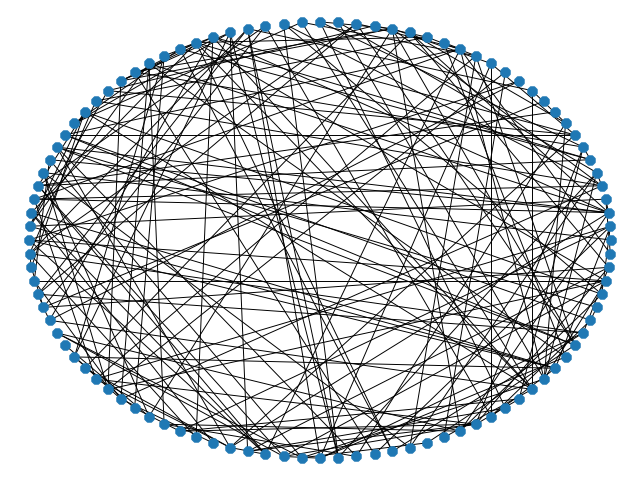
\includegraphics[width=0.85\textwidth]{img/plot.png}
    \caption{Example of graph visualization.}
    \label{ris:plot}
\end{figure}

The part of \textit{adjacency matrix}:

\begin{verbatim}
    [[0 0 0 ... 0 0 0]
     [0 0 0 ... 0 0 0]
     [0 0 0 ... 1 0 0]
            ...
     [0 0 1 ... 0 0 0]
     [0 0 0 ... 0 0 1]
     [0 0 0 ... 0 1 0]]
\end{verbatim}

The part of \textit{adjacency list}:

\begin{verbatim}
    0 {3, 69, 38, 27, 30}
    1 {50, 91}
    2 {97, 36, 73, 80, 16, 89, 26, 28}
    3 {0, 18, 29, 85}
    4 {26, 69}
    5 {32, 35, 9, 80, 21, 63}
    6 {12, 84, 86, 89, 62}
    7 {64, 99, 70, 20, 54, 90}
    8 {57, 20, 69}
    9 {91, 44, 5}
    10 {32, 49, 90}
\end{verbatim}

Advantages of the adjacency matrix:
\begin{itemize}
    \item complexity of checking for an edge between two vertexes: $O(1)$.
\end{itemize}

Disadvantages of the adjacency matrix:
\begin{itemize}
    \item it takes up $O(\lvert V \rvert^2)$ memory, which is unacceptable for sufficiently large graphs;
    \item complexity of iterating over all vertexes adjacent to a given vertex: $O(N)$.
\end{itemize}

Advantages of the adjacency list:
\begin{itemize}
    \item uses $O(\lvert V \rvert + \lvert E \rvert)$ memory, which is optimal;
    \item allows you to quickly iterate over the vertex's neighbors;
    \item allows you to check for an edge in $O(\log{N})$ and delete it.
\end{itemize}

Disadvantages of the adjacency list:
\begin{itemize}
    \item when working with saturated graphs (the number of edges is close to $V^2$), the speed $O(\log{N})$ may not be enough.
\end{itemize}

\begin{verbatim}
Use Depth-first search to find connected components of the graph and
Breadth-first search to find a shortest path between two random vertices.

[DFS] Connected components between nodes 38 and 93: [(38, 82), (82, 86), (86, 6),
    (6, 89), (89, 2), (2, 73), (73, 81), (81, 93)]
[BFS] Shortest path between nodes 38 and 93: [38, 64, 78, 93]
\end{verbatim}

Breadth-first search is less space efficient than depth-first search because BFS keeps a priority queue of the entire frontier while DFS maintains a few pointers at each level.

If it is known that an answer will likely be found far into a tree, DFS is a better option than BFS. BFS is good to use when the depth of the tree can vary or if a single answer is needed - for example, the shortest path in a tree.
If the entire tree should be traversed, DFS is a better option.

BFS always returns an optimal answer, but this is not guaranteed for DFS\@.

\subsection{Conclusion}\label{subsec:conclusion}

In this task, we applied and analyzed different representations of graphs and basic algorithms on graphs (Depth-first search and Breadth-first search).

\subsection{Appendix}\label{subsec:appendix}

The source code is located \href{https://github.com/vanSultan/anal_dev_algo/tree/lab_05}{here}: \url{https://github.com/vanSultan/anal_dev_algo/tree/lab_05}.
